\chapter{Unbounded team selection\label{chap:unbounded}}
Trainer Battles make very little use of random numbers (to the best of my
 knowledge, they only show up when checking for a Charged Attack side
 effect, and breaking CMP ties).
Their intrigue is rooted instead in ignorance: ignorance of
 the Pokémon you'll face, the order in which you'll face them,
 their statistics (beyond the static properties of the Species),
 their Attacks, and how their Trainer will employ them.

We've established that Pokémon battle fitness is dependent on opponent details.
We cannot name a globally superior Pokémon.
Primarily due to type effectiveness, there is no individual Pokémon that
  (assuming competent play by both Trainers) can defeat all others in even a
  1-on-1 contest.
Statistics based on some ``average opponent'' are fundamentally misleading.
Averages over the population do not correspond to any actual opponent,
 the population is more diverse than actual opponents,
 and current actual opponents cannot generally predict future opponents.
Even were this not the case, the situation into which a Pokémon is deployed
 can change drastically from match to match.
Accurate prediction comes not via stats, but simulation (\autoref{chap:simul}).

Yet the game provides a per-Pokémon ordered measure of strength in battle: Combat Power (CP).
Obviously no single statistic can account for all possible opponents, but
 we will see that CP is a very questionable assessment for a PvP
 context (and not great for PvE, either).

\section{Combat Power\label{sec:cp}}
A Pokémon's CP is defined as:
\[ CP = \max{10, \frac{Mod_A \times \sqrt{Mod_D} \times \sqrt{Mod_S} \times CPM^2}{10}} \]
CP growth is quadratic with respect to $CPM$, linear with $Mod_A$, and
  sublinear with $Mod_D$ and $Mod_S$.
Remember from our Damage equation that $Mod_A$ is divided by $Mod_D$
 to generate one of the factors.
This suggests that $Mod_D$ is undervalued by the CP equation, from which
 we might expect $Mod_A$ to be divided by $\sqrt{Mod_D}$.
MHP isn't used in the Damage equation, but knocking out a Pokémon
 requires inflicting some average Damage $D$ $n$ times,
 where $n = \lceil\frac{MHP}{D}\rceil$.
It is thus similarly undervalued by CP\@.
The quadratic term for CPM makes sense from the perspective of the Damage
 equation, since CPM is used as a factor when calculating Damage in the
 case of both the attacker and defender.
But since CPM is also used to calculate MHP from $Mod_S$, an argument
 can be made that it ought be raised to the third power.
Since $CPM < 1$ for all Levels, $CPM^3 < CPM^2$, and thus it seems \textit{overvalued} by CP\@.
Finally, recall that $MHP = \lfloor Eff_S \rfloor$.
Since the observable $MHP$ increases only stepwise with respect to $Eff_S$,
  there is a stepwise overvaluation of $Mod_S$.
This doesn't correct the undervaluation due the square root, but it does
  have effects: a 0/14/13 level 30.5 Clodsire has the same MHP
  as a 0/14/14 at the same level (213), but a CP of 1499 as
  opposed to the latter's 1502.
Despite being exactly the same on the field, one is allowed in Great League,
  and the other is prohibited.

Why would the game use such a flawed measure of power?
Clearly, a single stat was desired to cover both modes of Pokémon GO battling.
Since Raids allow substitution of defeated Pokémon, but are subject to a timer,
  the ability to defend and absorb Damage is less important than being able to
  quickly inflict damage.
Furthermore, when two Pokémon launch charged attacks on the same turn in a Trainer
  Battle, $Eff_A$ determines which goes first (\autoref{sec:3x3}).
Perhaps this explains the emphasis on attack, but some of the most important
  factors in the Damage equation are left out of CP entirely!
The Power and timing of the Pokémon's Attacks are not present, despite
  dominating the inflicted Damage and overall flow of the battle.
Type effectiveness and STAB have been likewise ignored, as have the
  properties of Shadow Pokémon.
It ought be clear that we must look beyond CP in our selection of Pokémon.

Remember that a type advantage is more impactful than a type
  disadvantage (60\% vs -37.5\%):
  all else being equal, it's usually more important to reduce your Pokémons'
  weaknesses than to increase their strengths.
Every typing is weak against at least one attack type---usually several.
Weakness against only a single type is uncommon: only seven typings manage it, and in two
 of those cases it's a double weakness (\autoref{table:singleweak}).
The only such typings with much population are Electric and Normal. 
\begin{table}[ht]
\centering
\begin{tabular}{ll}
Typing & Weakness\\
\Midrule
Bug+Steel & Fire (doubly weak) \\
Ghost+Normal & Dark \\
Dark+Ghost & Fairy \\
Dark+Poison & Ground \\
Electric & Ground \\
Ground+Water & Grass (doubly weak) \\
Normal & Fighting \\
\end{tabular}
  \caption{Single-weakness typings\label{table:singleweak}}
\end{table}

\section{How important are IVs?}
Well, how important are attack, defense, and stamina?
Every calculation that makes use of a Pokémon's base stats also uses the IVs.
In no universe will you benefit from paying IVs more attention than species statistics.
In bounded competition (see \autoref{chap:bounded}), higher IVs---just like higher
  base stats---are automatically counterbalanced.
This chapter is concerned with unbounded competition, and there IVs are more directly
  relevant, especially for CMP in mirror matches.

As with most such questions, we could answer ``the details are opponent-dependent'',
  declare the day done, and close up shop.
Somewhat vaguely, we might reply, ``they're worth a couple levels''.
More concretely, we can say ``they're more important with low base stats, less important
  with higher base stats''.
Quantitatively, we can say ``An $IV_A$ of 15 is worth more than STAB to an
  attacker with ATK less than 75. It is worth exactly as much (20\%) as STAB
  to an attacker with ATK of exactly 75. It is worth less than STAB
  to an attacker with ATK greater than 75.''
Similarly, an $IV_A$ of 15 is equal to type effectiveness of 1 when ATK is 25.
For a more plausible ATK of 150, a maximum $IV_A$ is worth a 10\% bonus to attack.

In general, $IV_A$ adds a percentage boost of

\[ \frac{IV_A}{ATK} \times 100 \]

\noindent{}to attack, and $IV_D$ lends the same (of course using DEF) to defense.

This might not lead to any change in actual damage, depending on
  an opponent's own attack and defense.
We can see this null effect in an opponent-independent way: it is quite possible
  for two different IVs to yield the exact same MHP.
As an example, a Sigilyph (base STA 176) at level 22 has an MHP of 119 with
  either a 15 or a 14 $IV_S$: there is literally no difference between the
  two values.
In short, IVs (usually) have real effects, but (especially for more powerful species)
  the difference between 0/0/0 and 15/15/15 is often less than that due to
  attack selection, type effectiveness, and strategy.

\section{Team assembly}
Does this extend to teams?
At first, it seems that it might: after all, a team's overall fitness
 depends on the entire opposing team, involving still more unknowns.
We will see that the team mechanism actually allows us to mitigate certain
 unknowns, while adding new ones.
Comparing teams is highly nontrivial, and this greater complexity admits
 further opportunities for strategy and cunning.

It's generally very bad if all three team members are weak to the same type.
Ideally, no two members share a type weakness.
Lead with a species having few/uncommon weaknesses, to avoid having to make the first switch.

You'll use fast attacks more than anything else, so their quality is critical.
There is little use for a Pokémon with bad fast attacks.
Attacks of shorter duration might be thought preferable to those requiring
  several turns, due to greater responsiveness.
In truth, experienced players ought comprehend the universe of possibilities
  within the timescale of a single fast attack.
Attacks of longer duration allow the opponent to blunder with regard to the
  timing of their charged attacks, but experienced players will avoid
  such errors.
Short attacks credit damage more quickly than long ones.
There's no general rule: fast attack selection comes down to attack type
  (both for effectiveness and STAB), the Pokémon's charged attacks,
  and even the $\frac{P \times Eff_A}{Eff_D}$ of expected opponents.
Some Pokémon can learn two fast attacks of the same type and duration,
  where one is strictly inferior to the other in terms of power and
  energy.
Such garbage attacks ought be immediately changed with a Fast TM\@.

\begin{tipbox}[title=Dubwool+Wooloo+Mareep is a BAA team]
You'll hear a lot of bafflegab about ABA teams and ABB teams and CBD teams.
  In my opinion, these terms are somewhat useful for characterizing teams
  (the chained team from \autoref{chap:strategy} would be an ABC team),
  but they're not design principles, per se.
Build a team around the Pokémon, not acronyms.
\end{tipbox}

Each Pokémon ought know two charged attacks.
Ought they be of different types?
Some say that if they are of the same type, you can select for either time or power, depending on context.
This remains true, however, if they are of different types; the power simply depends on
  the different type relations.
It might indeed be that the more expensive charged move with higher PPE is no
  longer advantageous (if it is ineffective, and the other move is not),
  but it might also be the case that it is even more advantageous,
  or the cheaper move is now more powerful.
Either way, I consider wider type effectiveness to be more important than gains in PPE;
  after all, it is rare that two quality charged moves are separated by a PPE factor
  of 1.6 \textbf{verify this}!
It is best if they are not both ineffective against any typing, and one or the
  other is effective against many typings.
Remember, unlike defense, adding attack types can only be beneficial.
Pokémon that can't learn two good charged attacks having distinct types are best avoided.

\section{Solving Pokémon PvP}
If there exists a subgraph including the root of the game tree such that at each
  node it includes all choices from Trainer $A$ for at least one choice from Trainer $B$
  (Trainer $B$'s choice can of course be different at different states), and all
  paths terminate in victory for Trainer $A$, Trainer $A$'s team can be considered
  to \textit{dominate} the team of $B$---assuming perfect play from $A$ (defined
  as a path in such a subgraph), $B$ is condemned to lose, no matter their choices.
We consider finding such a team $A$ to be a ``solution'' for the problem presented
  by team $B$.
Does there exist a team that dominates all possible teams?

Almost certainly not.
At the unbounded top end, or the top end under a capability bound (\autoref{chap:bounded}), Pokémon are not generally
  wildly superior to one another, nor are their attacks.
Gains of 1.6x are infrequent; it is rare that one can overcome type
  effectiveness with stats alone, whether they be attack, defense, or stamina.
Since every typing has weaknesses, a team can be constructed with
  very effective attacks against all possible orderings of any three Pokémon,
  and the former team is likely to dominate the latter.

Consider how your team would play against a team of the same or similar composition (simulation
  is invaluable---see \autoref{chap:simul}).
Perturb your selections, replacing them with ideal counters.
Develop an ideal team for facing your team, then an ideal team for facing that team.
Does this process converge?
\vfill
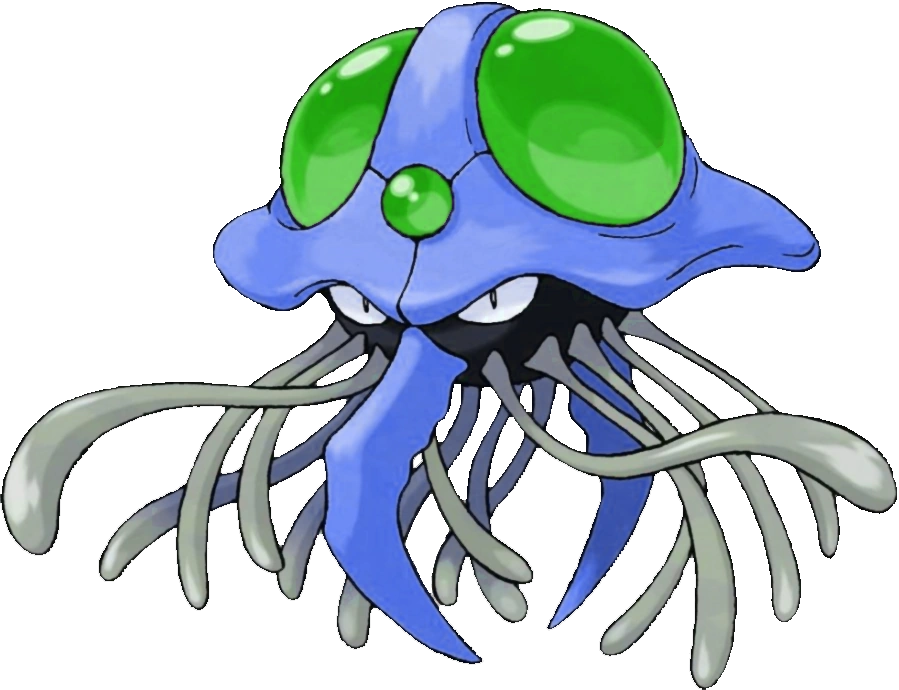
\includegraphics[width=.9\linewidth,keepaspectratio]{images/tentacruel.png}
